\chapter{Identyfikacja}
Zdecydowano się zaprezentować tylko rozmyte modele w wariancie rekurencyjnym, tzn. modele nie korzystają z pomiarów obiektu, a jedynie bazują na wyjściach modelu.

\section{Model Hammersteina}

\begin{figure}[h!]
\centering
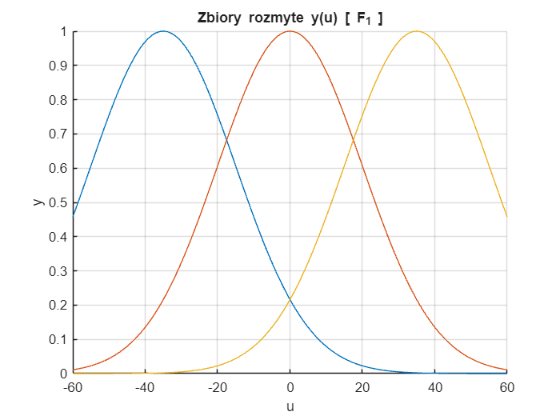
\includegraphics[width=0.6\textwidth]{pictures/fuzzy_hamm_f1}
\caption{Rozmyte sterowanie $F_1$ - model Hammersteina, następniki nieliniowe.}
\end{figure}

\begin{figure}[h!]
\centering
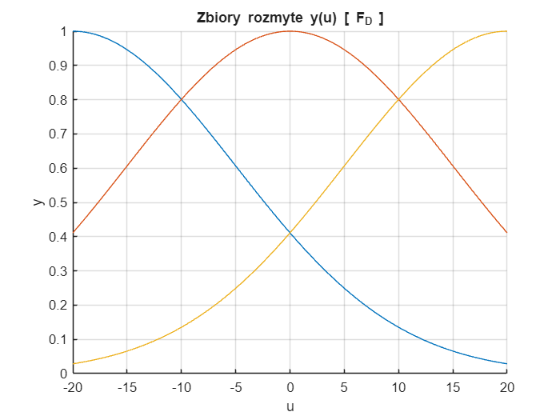
\includegraphics[width=0.6\textwidth]{pictures/fuzzy_hamm_fd}
\caption{Rozmyte zakłócenie $F_D$ - model Hammersteina, następniki nieliniowe.}
\end{figure}

\newpage

\begin{figure}[h!]
\centering
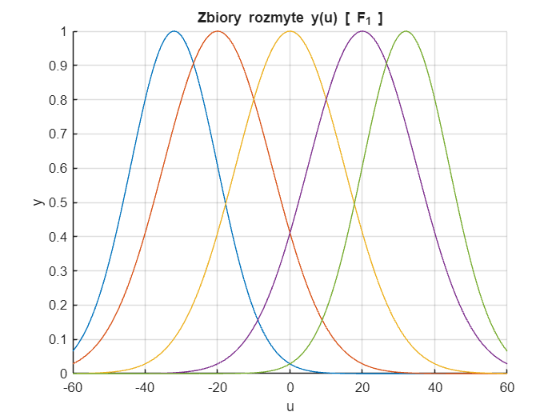
\includegraphics[width=0.8\textwidth]{pictures/fuzzy_hamm_f1_lin}
\caption{Rozmyte sterowanie $F_1$ - model Hammersteina, następniki liniowe.}
\end{figure}

\begin{figure}[h!]
\centering
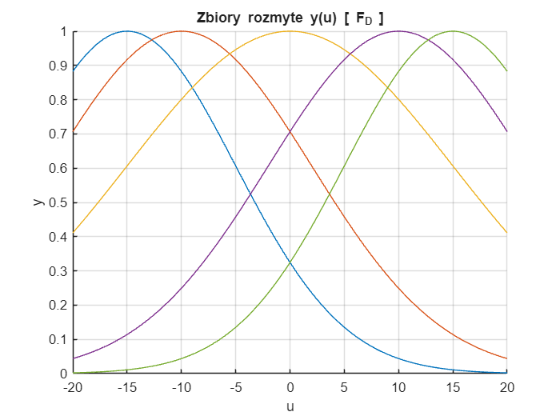
\includegraphics[width=0.8\textwidth]{pictures/fuzzy_hamm_fd_lin}
\caption{Rozmyte zakłócenie $F_D$ - model Hammersteina, następniki liniowe.}
\end{figure}

\newpage

\section{Model Wienera}

\begin{figure}[h!]
\centering
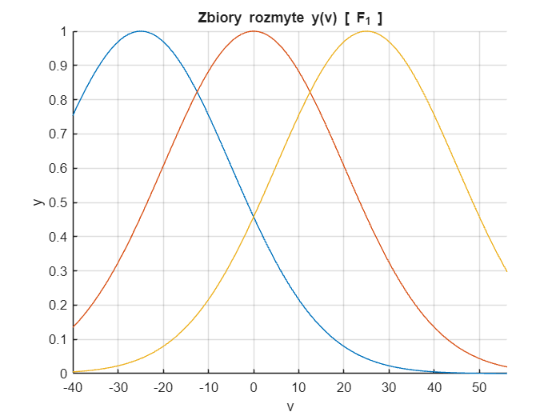
\includegraphics[width=0.8\textwidth]{pictures/fuzzy_wien_f1}
\caption{Rozmyte sterowanie $F_1$ - model Wienera, następniki nieliniowe.}
\end{figure}

\begin{figure}[h!]
\centering
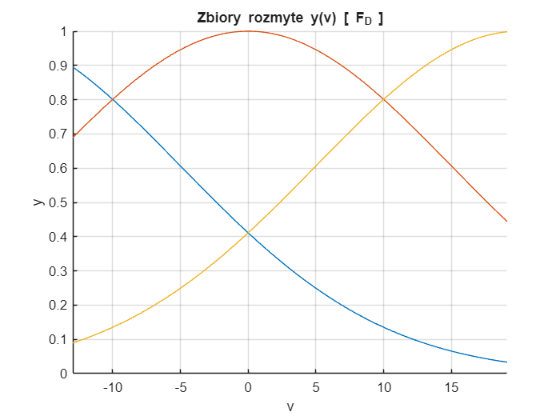
\includegraphics[width=0.8\textwidth]{pictures/fuzzy_wien_fd}
\caption{Rozmyte zakłócenie $F_D$ - model Wienera, następniki nieliniowe.}
\end{figure}

\newpage

\begin{figure}[h!]
\centering
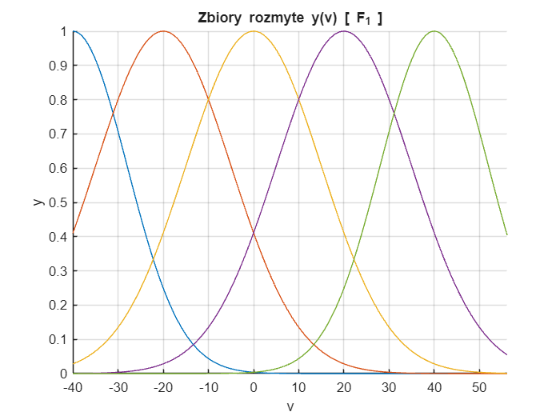
\includegraphics[width=0.8\textwidth]{pictures/fuzzy_wien_f1_lin}
\caption{Rozmyte sterowanie $F_1$ - model Wienera, następniki liniowe.}
\end{figure}

\begin{figure}[h!]
\centering
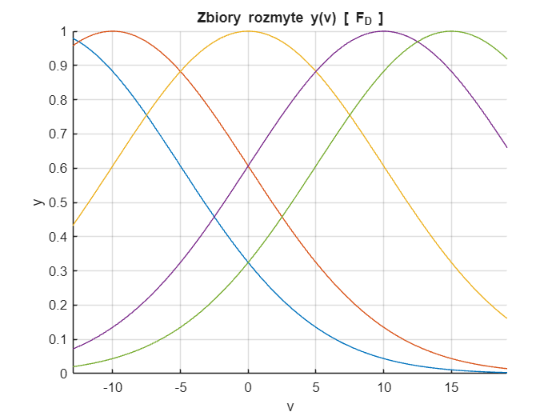
\includegraphics[width=0.8\textwidth]{pictures/fuzzy_wien_fd_lin}
\caption{Rozmyte zakłócenie $F_D$ - model Wienera, następniki liniowe.}
\end{figure}

